\subsection{Pixhawk and HiL}
\label{sec:Pixhawk_and_HiL}


\subsubsection{Sensorrauschen und Kalmann Filter}
Hierbei handelt es sich \textbf{nicht} um eine HiL Simulation, sondern um einen ersten, einfachen Testaufbau mit funktionierender Datenübertragung zwischen Pixhawk und Simulink als Host PC. 

\begin{figure}[ht]
  \begin{center}
  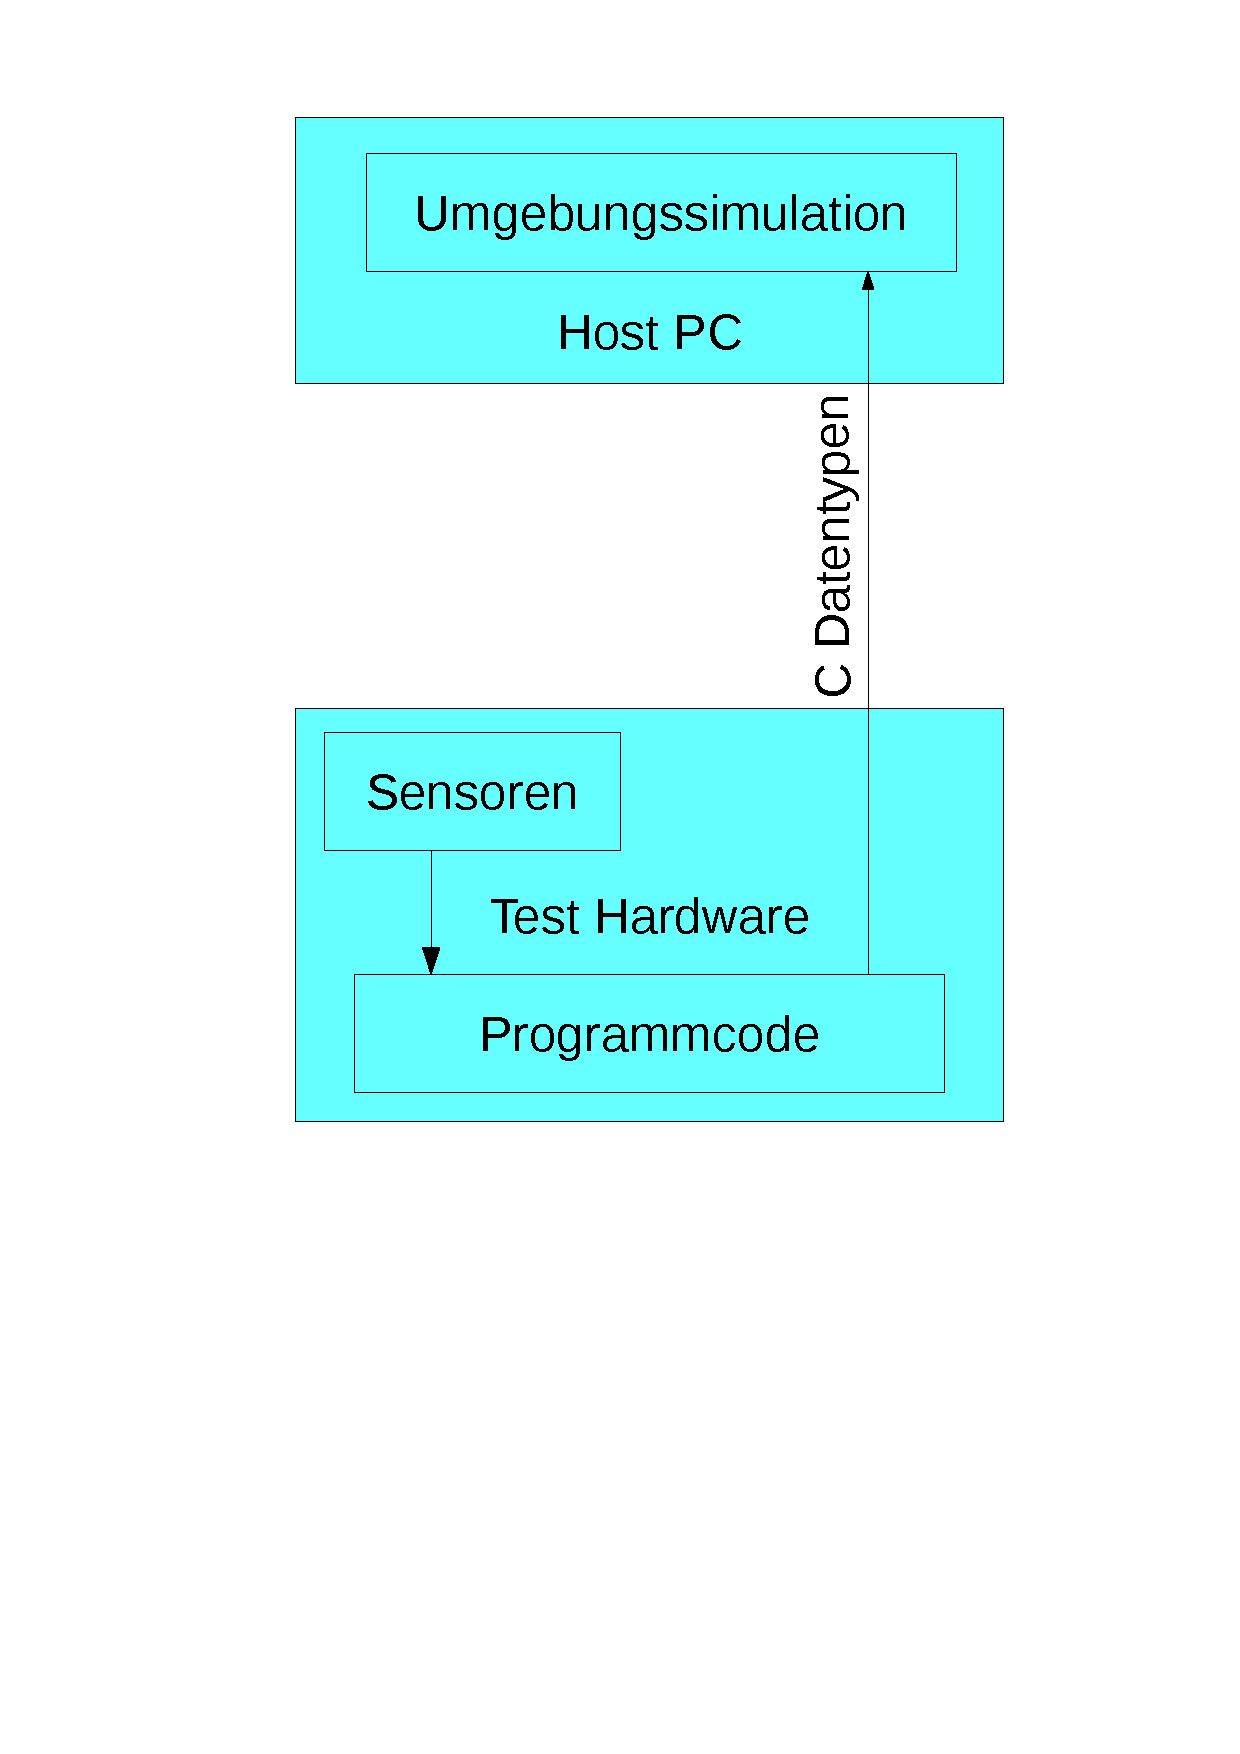
\includegraphics[scale=0.5, trim={5cm 10.6cm 2.5cm 2cm},clip]{pic/35_hil/hil_sensor_noise.pdf}
  \caption{Messung Sensorrauschen}
  \label{fig:messung_sensorrauschen}
  \end{center}
\end{figure}

\noindent Die Sensordaten wie Gyro-, Accelero-, Barometer und Temperaturfühler werden von der Test Hardware entgegengenommen. Diese Daten durchlaufen einen Kalmann Filter und liegen dann als roh-, sowie gefilterte Werte auf der uORB zur Weiterverarbeitung. Diese Werte werden dann im Programmcode abgegriffen und über eine serielle Schnittstelle an den Host PC übermittelt.\\
Auf dem Umgebungssimulator kann nun ein Kalmann Filter auf die roh Werte angewendet werden und mit den gefilterten Werten verglichen.



\subsubsection{Systemtest 1}
In einem weiteren Test könnte die Flugsteuerung vom Pixhawk getestet werden wie in Abbildung \ref{fig:hil_pixhawk} aufgezeigt. Die Datenübertragung wäre weiterhin auf einer seriellen Schnittstelle. Daruch wäre eine komplette HiL Simulation möglich.

\subsubsection{Systemtest 2}
Eine weitere Möglichkeit wäre, vorhandene Sensorwerte eines aufgezeichneten Flugs in the uORB einzuspeisen. Die berechnete Rotorenstellgrösse vom Pixhawk könnte man anschliessend mit den vorhandenen Aktuatorenwerten vergleichen.
\clearpage